We used the Pima Indians Diabetes Dataset from the National Institute of Diabetes and Digestive and Kidney Diseases. This dataset has a binary response variable indicating if the sample has diabetes and eight covariates on 768 samples. The data was standardized to have mean zero and standard deviation one.\\

We can see that using the Hamiltonian Monte Carlo algorithm produced good mixing with energy decreasing downwards and converging:

\begin{figure}[H]
	\centering
	\begin{minipage}{0.45\textwidth}
		\centering
		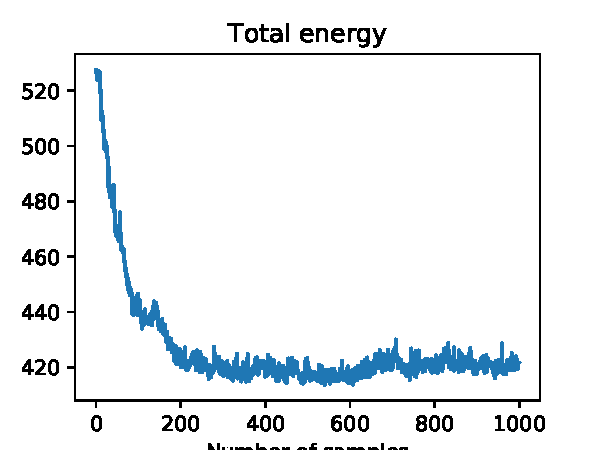
\includegraphics[width=0.9\textwidth]{hmc-energy-pima.pdf} % first figure itself
		\caption{first figure}
	\end{minipage}\hfill
	\begin{minipage}{0.45\textwidth}
		\centering
		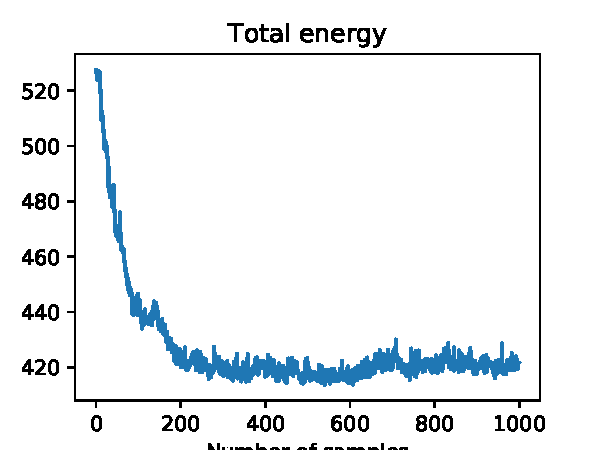
\includegraphics[width=0.9\textwidth]{hmc-energy-pima.pdf} % second figure itself
		\caption{second figure}
	\end{minipage}
\end{figure}

We can see that using the Stochastic Gradient Hamiltonian Monte Carlo algorithm produced good mixing with energy decreasing downwards and converging:

\begin{figure}[H]
	\centering
	\begin{minipage}{0.45\textwidth}
		\centering
		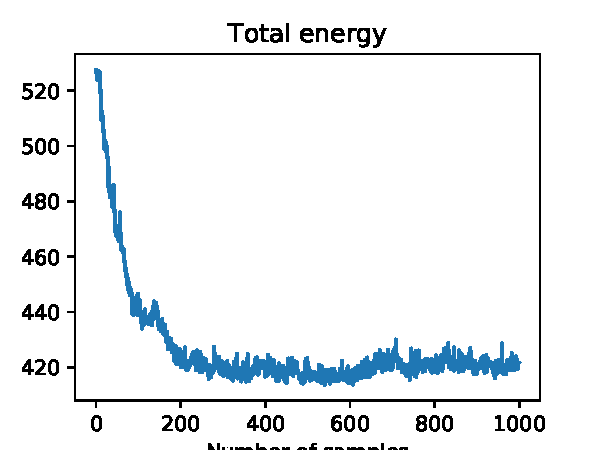
\includegraphics[width=0.9\textwidth]{hmc-energy-pima.pdf} % first figure itself
		\caption{first figure}
	\end{minipage}\hfill
	\begin{minipage}{0.45\textwidth}
		\centering
		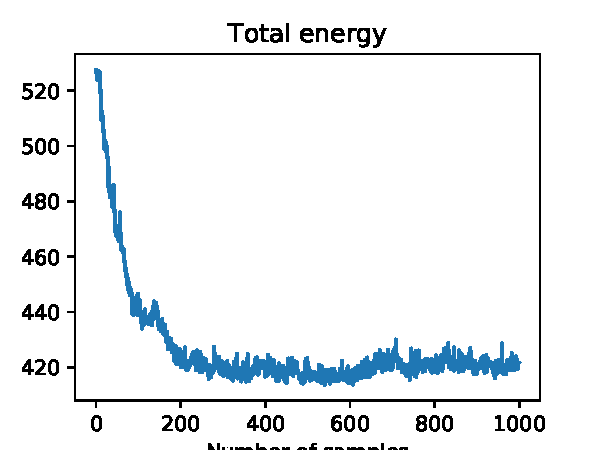
\includegraphics[width=0.9\textwidth]{hmc-energy-pima.pdf} % second figure itself
		\caption{second figure}
	\end{minipage}
\end{figure}


We compared the coefficients produced by each algorithm to the MLE estimates to check for accuracy:

\begin{figure}[H]
	\centering
	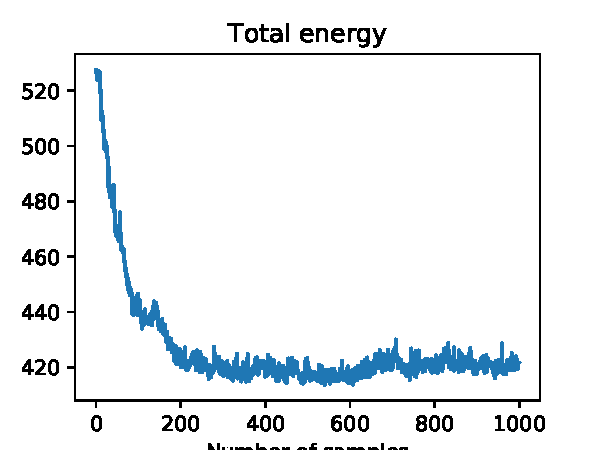
\includegraphics[width=0.45\textwidth]{hmc-energy-pima.pdf}
\end{figure}

